Os dados abaixo são parciais de um levantamento de músicas no \textit{Soundcloud} utilizando palavras-chave\footnote{No sentido de um parâmetro de procura em \emph{Query-strings}; para mais informações, ver \url{https://en.wikipedia.org/wiki/Query_string}} relativas à produção da prática discutida neste trabalho organizadas em categorias de informação.

\emph{Palavras-chave} são os termos que apresentaram maior consistência de dados (considerados pelo ponto de vista abstrato do autor do trabalho): \begin{inparaenum}[\itshape a)\upshape]
\item \emph{algorave}/\emph{algopop}: parte considerável da produção do \emph{livecoding} realizada em ambientes noturnos, informais ou de entretenimento (possue relação com o elemento dança);
\item \emph{livecoding}/\emph{live-coding}: apresentaram dados coerentes com a bibliografia pesquisada\footnote{A exclusão do termo \emph{live code/live coding} foi feita pois a separação criava uma ambiguidade de busca no \emph{Soundcloud}, isto é, \emph{live} poderia não se referir ao que pesquisamos por \emph{livecoding}.};
\item \emph{bytebeat}: parte considerável de uma técnica de programação musical descrita pela primeira vez por \citeonline{heikkila_discovering_2011} e aplicada no \emph{livecoding}, isto é, apenas um fragmento dessa prodção pode se encaixar como \emph{livecoding} (um desses programas é o \emph{Wavepot});
\item \emph{algorithmic music}: utilizei o termo para apontar o quanto da música algorítmica publicada no \emph{Soundcloud} poderia ser classificado como \emph{livecoding}, em conjunto com outros termos que não foram abordados nesta pesquisa;
\item \emph{wavepot}: performances feitas com o aplicativo \emph{Wavepot}, são por definição \emph{livecoding};
\end{inparaenum}

Categorias de informação são:\begin{inparaenum}[\itshape a)\upshape]
\item ano de publicação (\emph{created\_at});
\item países (\emph{country});
\item cidade (\emph{city});
\item gênero musical(\emph{genre});e 
\item licensa de uso (\emph{license})
\end{inparaenum}

\section{Plotagem em forma de torta}

Os dados foram levantados entre janeiro e fevereiro de 2015; não realizamos desde então levantamentos por utilizarmos um outro sistema de visualização. Estão disponíveis na \autoref{apend:torta}

\section{Plotagem em forma de círculos empacotados}\label{dados_pacotao}

Os dados utilizados são os mesmos. A diferença é o tratamento dos dados: correlação de dados por duas categorias diferentes. Nos exemplos abaixo, salientei comparações de ano e gênero (\autoref{pacotao} e \autoref{pacotao2}) e país e gênero (\autoref{pacotao3} e \autoref{pacotao4}).

\begin{figure}
\begin{center}
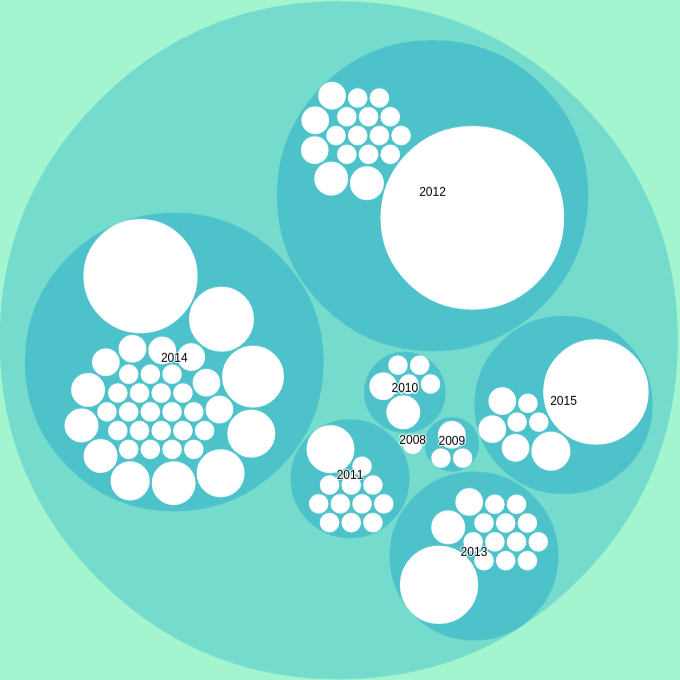
\includegraphics[scale=0.6]{./imagens/zoomable_circle_packing_genre_year_livecoding.png}
\caption{Empacotamento de informações a respeito de gênero musical a partir de anos de produção}
\label{pacotao}
\end{center}
\end{figure}

\begin{figure}
\begin{center}
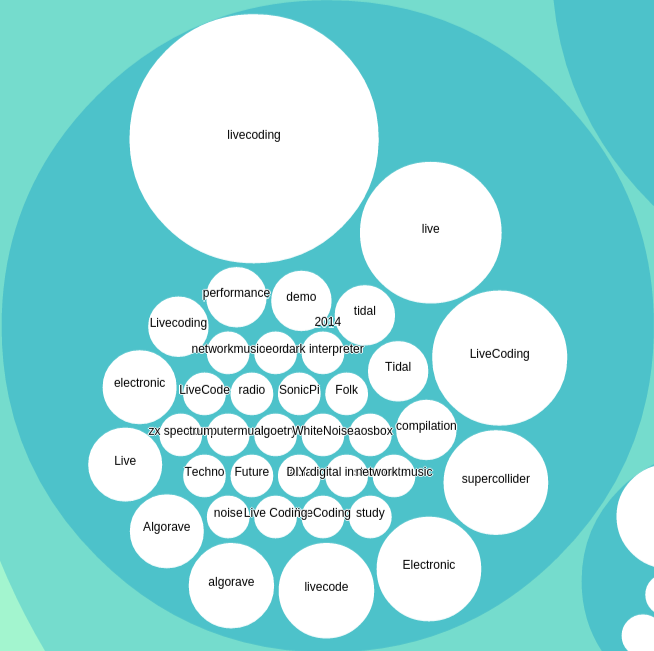
\includegraphics[scale=0.6]{./imagens/zoomable_circle_packing_genre_year_livecoding2.png}
\caption{Detalhamento de informações a respeito de gênero musical a partir de anos de produção}
\label{pacotao2}
\end{center}
\end{figure}

\begin{figure}
\begin{center}
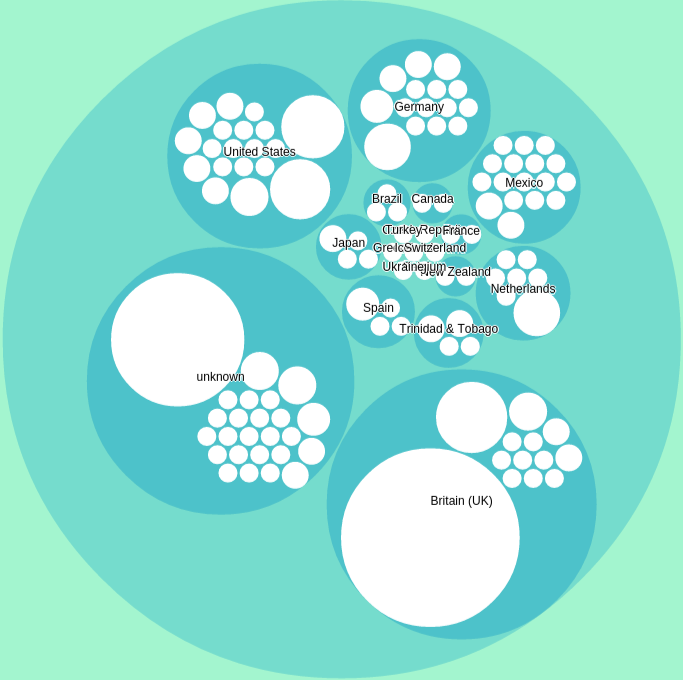
\includegraphics[scale=0.6]{./imagens/zoomable_circle_packing_genre_year_livecoding3.png}
\caption{Empacotamento de informações a respeito de gênero musical a partir de países onde ocorreram as produções}
\label{pacotao3}
\end{center}
\end{figure}

\begin{figure}
\begin{center}
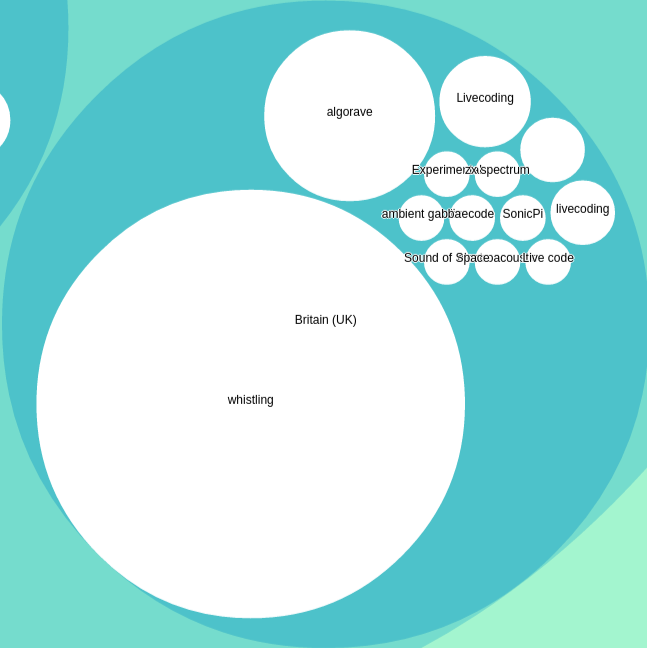
\includegraphics[scale=0.6]{./imagens/zoomable_circle_packing_genre_year_livecoding4.png}
\caption{Detalhamento de informações a respeito de gênero musical a partir de países onde ocorreram as produções.}
\label{pacotao4}
\end{center}
\end{figure}



